\subsection{Particle Indentification}
 
 The goal of cuts efficiency study is to obtain most optimized cut values on PID detectors to reject most of background particles (mainly pions) while keeping as more electrons as possible. The kinematic settings of E08014 experiemnt determine that the production of pions is much rare comparing with scattered electrons, and the new trigger design also has already removed most of pions during online data taking by intruducing GC detectors in the trigger system, so we are supposed to have high cut efficiencies and very small pions contamination. 
 
 Events from T6 and T7 triggers were used to study the PID cut efficiencies since they contain more pions. Acceptance cuts and VDCs One-Track cuts were also applied to eliminate cosmic ray events and multi-scattering electrons. Then pure pion samples and pure electrons samples were chosed from Calorimeters (GC) when we studied cut efficiency of GC (Calorimeters). The percentages of pions and electrons left over after cutting GC (Calorimeters) are called pion rejection efficiency and electron cut efficiency, respectively, and the definitions are given by:

\begin{equation}
 \epsilon_{pion\_rej}^{cer(calo)} = \frac{N_{pion\_after\_cut}^{cer(calo)}}{N_{pion\_samples\_from\_calo(cer)}},  \epsilon_{electron\_cut}^{cer(calo)} = \frac{N_{electron\_after\_cut}^{cer(calo)}}{N_{electron\_samples\_from\_calo(cer)}},     
    \end{equation}


 A procedure of cut scanning is to obtain pion rejection efficiency and electron cut efficiency, then to determine most suitable cut values. Fig~\ref{Lgc_eff} and Fig~\ref{Rgc_eff} shows that cutting on low channels (50) of GC ADC sum can already remove most of pions while keep more than 99\% of electrons. The combination  cuts on E/P (0.5 on both arms) and the second layer ADC sum of Calorimeters (100 for PRL2 and 200 for Shower) will further remove above 90\% of pions while still above 99\% of electrons remaining (Fig~\ref{Lcalo_eff} and Fig~\ref{Rcalo_eff}). Totally for data in HRS-L and HRS-R, 99.85\% (99.62\%) of pions are eliminated with PID cuts, and meanwhile, 99.58\% and 99.86\% of electrons surivive after the cuts. Considering the high electrons rates and low pion production for our kinematics, we don't need special corrections of pion contaimination.

\begin{figure}[h!]
\centerline{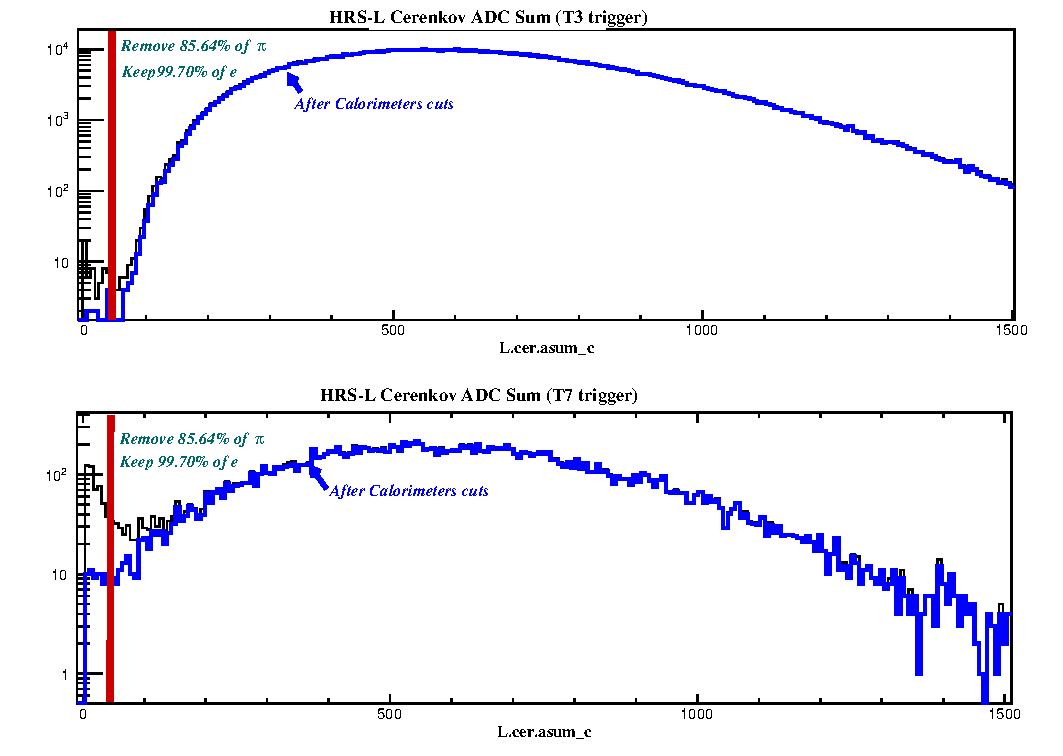
\includegraphics[width=0.8\linewidth]{figures/pid/L_Cer_PID_Cut.eps}}
\caption[GC cut efficiencies on HRS-L]{\footnotesize{GC cut efficiencies on HRS-L}}
\label{Lgc_eff}
\end{figure}

\begin{figure}[h!]
\centerline{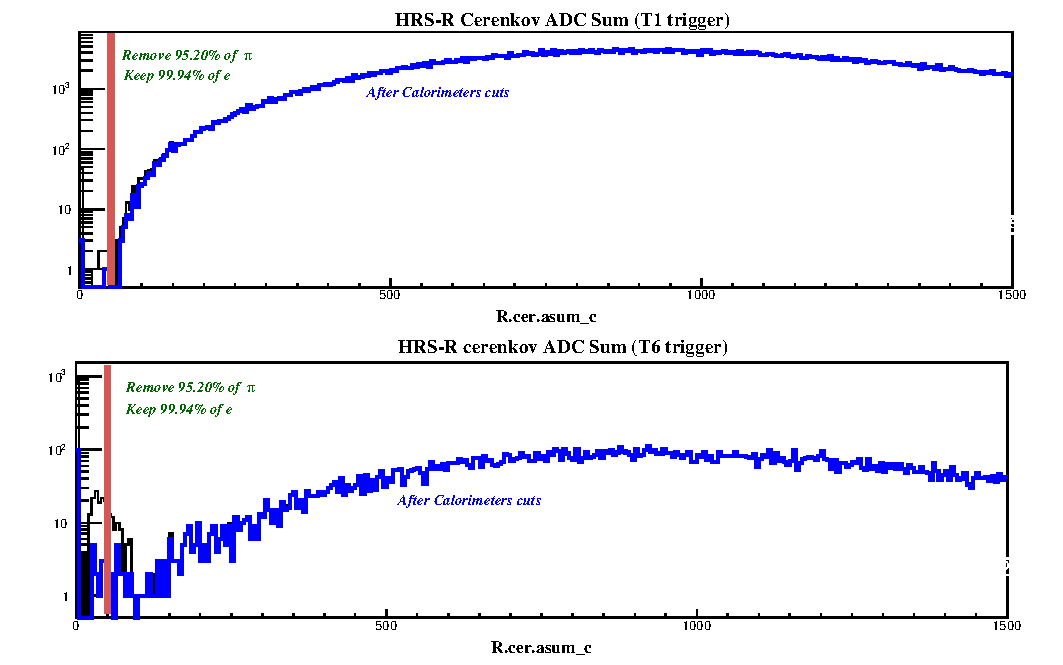
\includegraphics[width=0.8\linewidth]{figures/pid/R_Cer_PID_Cut.eps}}
\caption[GC cut efficiencies on HRS-R]{\footnotesize{GC cut efficiencies on HRS-R}}
\label{Rgc_eff}
\end{figure}

\begin{figure}[h!]
\centerline{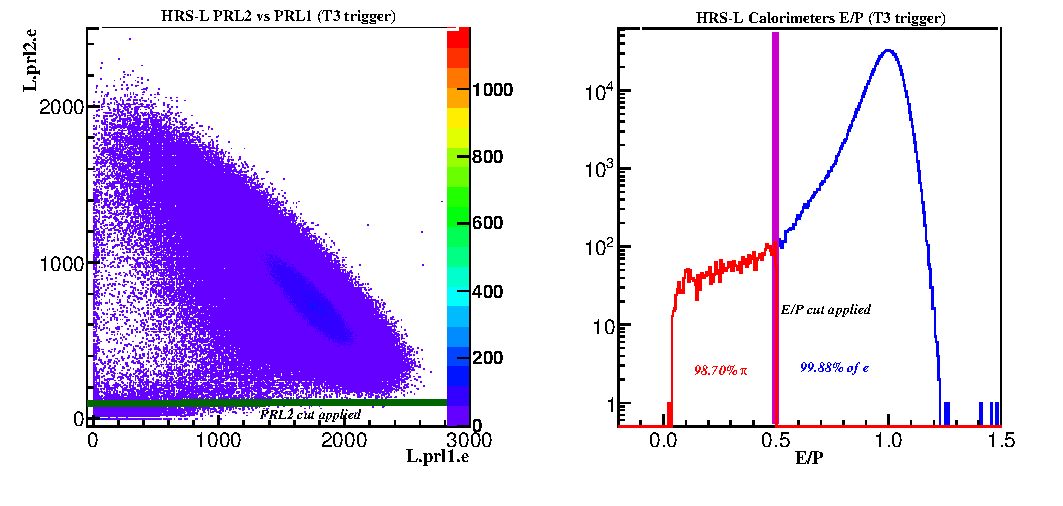
\includegraphics[width=0.8\linewidth]{figures/pid/L_Calo_PID_Cut.eps}}
\caption[Calorimeters cut efficiency on HRS-L]{\footnotesize{Calorimeters cut efficiency on HRS-L}}
\label{Lcalo_eff}
\end{figure}

\begin{figure}[h!]
\centerline{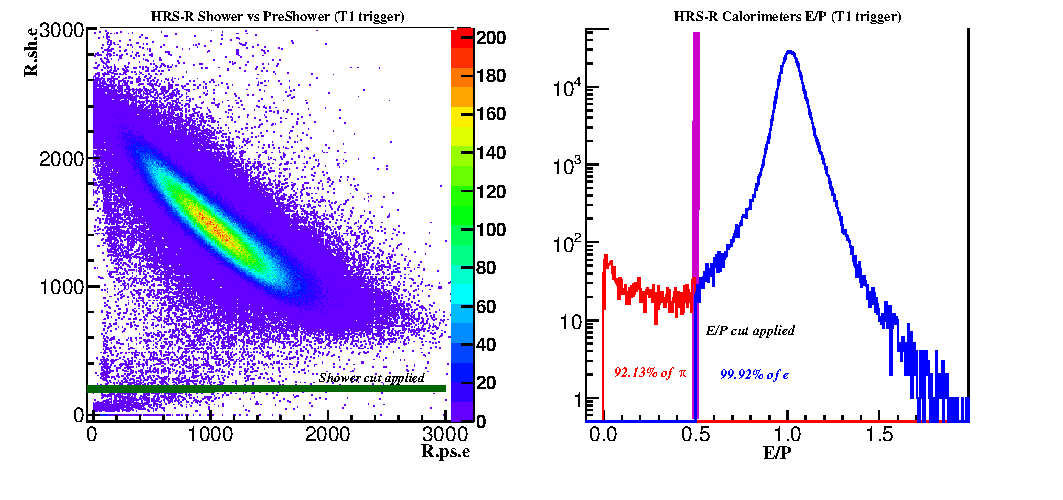
\includegraphics[width=0.8\linewidth]{figures/pid/R_Calo_PID_Cut.eps}}
\caption[Calorimeters cut efficiency on HRS-R]{\footnotesize{Calorimeters cut efficiency on HRS-R}}
\label{Rcalo_eff}
\end{figure}

As we discuss in the previous section, values of cut efficiencies should be corrected by detection efficiencies of the detectors since pion and electron samples from other detectors are not necessarily detected by the detectors due to their inefficiencies. Because detection efficiencies don't relate to particle types, pion rejection efficiency and electron cut efficiency should correctly redefined as:
 
\begin{equation}
 \epsilon_{pion\_rej}^{cer(calo)} = \frac{N_{pion\_after\_cut}^{cer(calo)} \cdot \epsilon_{det}^{cer(calo)}}{N_{pion\_samples\_from\_calo(cer)}},  \epsilon_{electron\_cut}^{cer(calo)} = \frac{N_{electron\_after\_cut}^{cer(calo)} \cdot \epsilon_{det}^{cer(calo)}}{N_{electron\_samples\_from\_calo(cer)}},        
\end{equation}

 The detection efficiencies of PID detectors in Hall-A are near 99.9\% as we discussed in the previous section so we don't correct the values of PID cut efficiencies. 